\chapter{FPGA}
\label{chap:fpga}
A powerful Virtex-7 \gls{FPGA} Evaluation board VC707
was used to for real time signal processing.
For experiments performed in this thesis
the data from the \gls{ADC} is acquired, stored in real time
and than passed to Matlab running on a personal computer.
This allows to both analyze the analog part of the system
while keeping the fast implementation speed and flexibility of Matlab
to test of the digital signal processing steps of the receiver.
Nevertheless the architecture was chosen such, that it is now easy
to step by step move parts of the signal processing from Matlab to the
\gls{FPGA}. \\

\section{Architecture Overview}
The three main tasks of the digital design are first to interface
the \gls{ADC} and acquire its data, then to store it on a
\gls{DDR} \gls{RAM} and finally to allow a computer to
slowly download it. \\

As shown in \figref{fig:fpga_architecture_overview} the most important
modules of the design are the Adc12d1800 which interfaces the
\gls{ADC}, Ram which uses a \gls{DDR}3-\gls{RAM} to store the data
and Microblaze, a soft-core processor, which controls the
\gls{USB} 2 data download. Data2Ram is interface logic used
to connect the \gls{ADC} directly to the \gls{RAM}. Later the receiver logic,
starting with frame synchronization could be implemented
at this place. AxiSlave implements an interface between the
\gls{AXI}-Bus used by the Microblaze processor and the custom
Ram module. \\

In the following sections, each of this modules is shortly described followed
by some insights how clocking and reset is implemented. \\

\begin{figure}[ht]
  \centering
  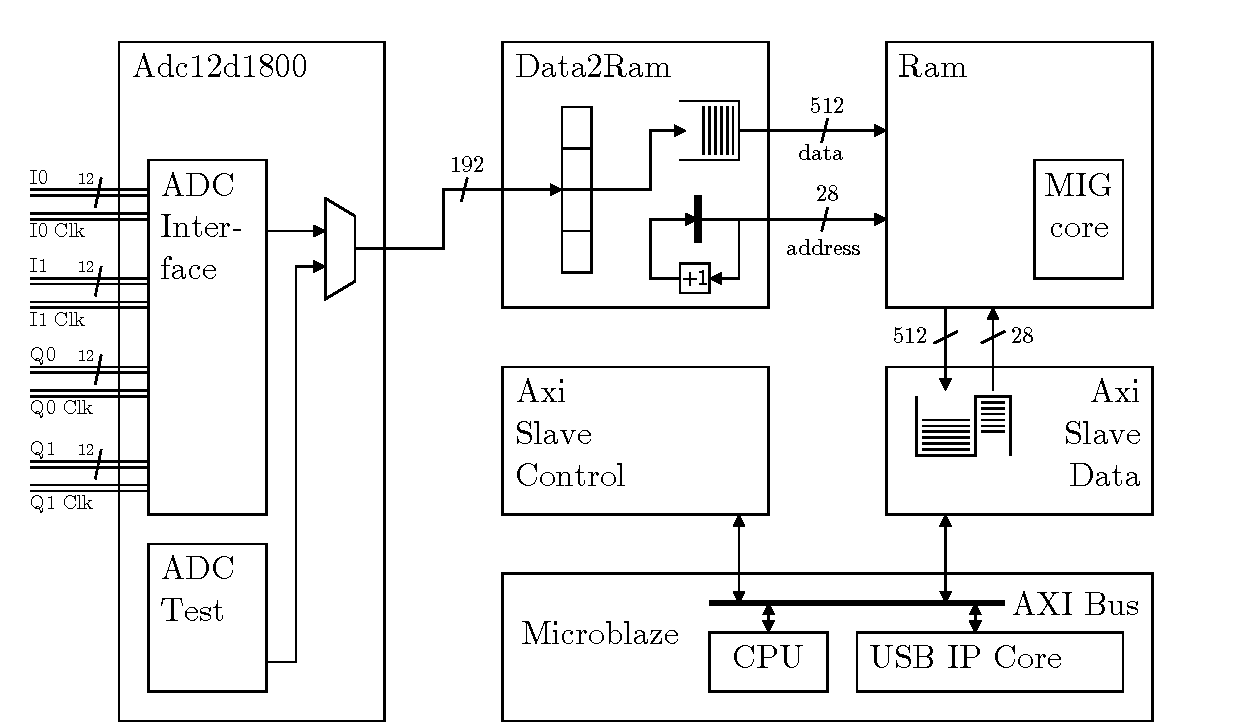
\includegraphics[width=\textwidth]{figures/fpga_architecture_overview}
  \caption{Overview of the architecture}
  \label{fig:fpga_architecture_overview}
\end{figure}

\section{Data Flow Model}
\label{sec:fpga_reqack}
Between most modules, a simple communication protocol is used that allows
one way communication whenever the sender and the receiver are both
ready. As a consequence all modules have to be stallable. By only using
one such protocol arbitrary modules can often be connected
without any additional glue logic. \\

The protocol requires the sender to provide a \acrfull{req} output, which
is asserted if it has data to send. The receiver provides a \gls{ack}
output to confirm that it is ready to receive the data.
Acknowledge can only be applied when \gls{req} is asserted.
Data is transferred whenever there is a positive clock edge and
\gls{req} and \gls{ack} are both asserted (high). \\

Because the \gls{ack} output of a receiver by definition always depends on the
\gls{req} input of a receiver, this can result in long chains of routing and
\gls{LUT} resources when connecting multiple such modules.
Therefor a simple so called \gls{req}/\gls{ack}-breaker is used, which adds one
register into the data path. This results in one cycle delay but makes the
\gls{ack} signal depending on a local register only and not on the
\gls{req} signal. \\

This \gls{req}/\gls{ack}-breaker also allows for signals to be propagated
far across the die by separating long routing distances into smaller
ones by inserting registers into the data and control path. \\

\section{Data Acquisition}
\label{sec:fpga_adc}

The \gls{ADC} Reference Board (see \secref{sec:comp_adc}) is connected
to the Virtex-7 evaluation board (see \secref{sec:comp_virtex7})
using one of the two \gls{FMC} plugs.
A listing of all connections can be found in \appref{app:app_adc_fpga_con}. \\

Data acquisition is done by the module Adc12d1800. In our case the ADC is
configured to sample two channels, an in-phase and a quadrature phase channel,
at up to 1.8 GHz or to sample one channel at 3.6 GHz.
The nominal resolution is 12 bits. This results in a total bandwidth of
$5.4 \text{GB}/\text{s}$. \\
Since 1.8 GHz and especially 3.6 GHz is far beyond what the IO-Pads of all
\glspl{FPGA} \todo{reference needed} and most \glspl{ASIC} can handle,
the ADC can output on 4 parallel streams of 12 bits each. \\

Since this 4 streams might be routed with different wire lengths on a \gls{PCB}
each stream has it's own clock, which is aligned to the data.
In order to half the maximum frequency of the clock lines,
the data change on positive and negative clock edges (\gls{DDR}). \\

At full speed, this results in a switching frequency of 450 MHz for all data
and clock lines. To support this high speed, \gls{LVDS} signaling is used,
which reduces power consumption and the influence of noise
compared to classical \gls{CMOS} signaling. \\

Since the maximum clock frequencies of the Virtex \glspl{FPGA} for logic
including \gls{LUT} slices and medium to high fan-outs
are limited to around 200 to 300 MHz, the input stream needs to be further
parallelised. This design uses a frequency of 250 MHz to output
the data of the \gls{ADC} for further processing. At this frequency
only $4\;\text{ns}$ are available between clock edges, which is exceeded
easily as soon as a signal is routed far across the \gls{FPGA} die,
has a fan-out of more than about 4, when crossing clock domains, which lead
to clock skew, or by more than about 3 logic slices between registers.
This makes the \gls{FPGA} design challenging since often multiple
complete synthesis, map, place \& route and timing analysis runs are
needed to find a design that meets timing constraints. \\

As shown in \figref{fig:fpga_adc}, the implemented design uses
a total of 4 stages to parallelise and centralize the data to
one single data stream. \\

\begin{figure}[ht]
  \centering
  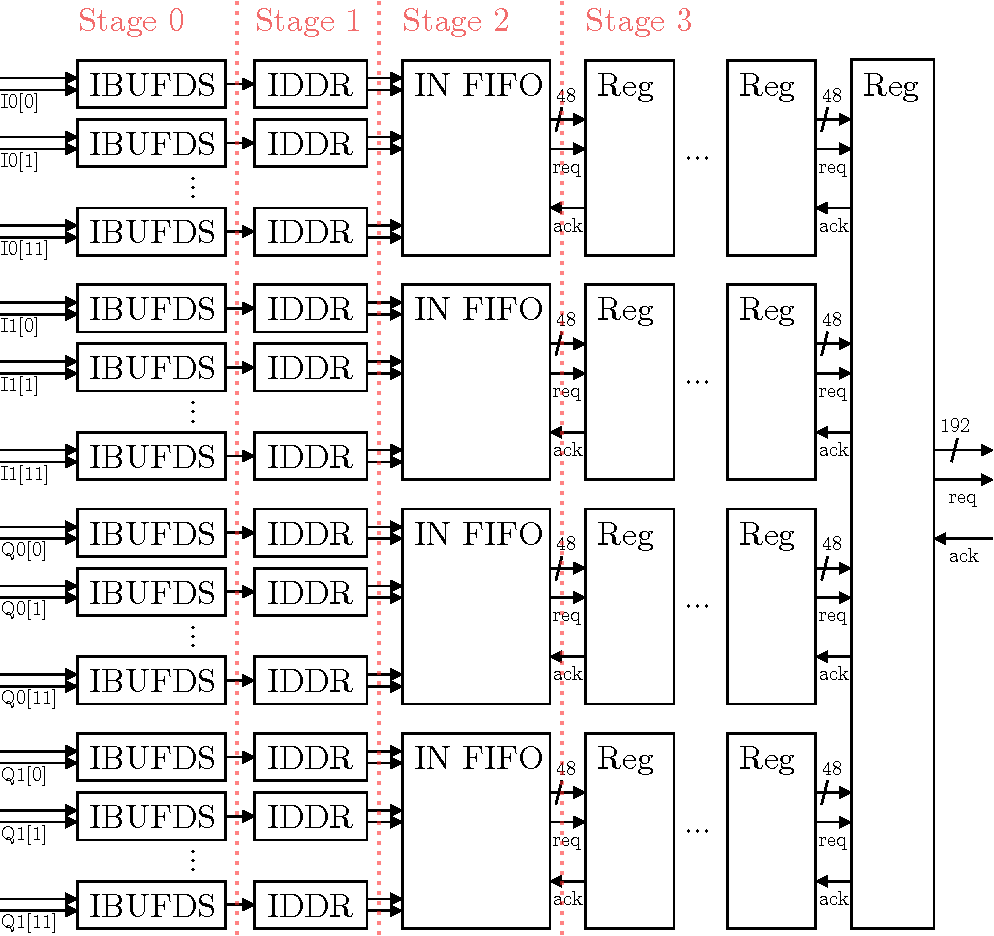
\includegraphics[width=\textwidth]{figures/fpga_adc}
  \caption{Data path of the \gls{ADC} module}
  \label{fig:fpga_adc}
\end{figure}

\subsection{Stage 0: Differential to Single-ended Conversion}
Each of the 12 bits and the clock of the 4 streams arrive at at the input bank
of the \gls{FPGA} at two neighbouring pads forming a \gls{LVDS} pair.
First this differential signal is converted to a single ended signal using
\gls{IBUFDS} primitives located next
to the pads. \\

This results in $4 \times 12$ bits of single ended, double data rate
signals plus 4 single ended clocks at up to 450 MHz. \\

\subsection{Stage 1: Double Data Rate to Single Data Rate Conversion}
\label{sec:fpga_adc_s1}
Next the first parallelisation step is performed by outputting two new
bits on every positive clock edge, instead of one on positive and one on
negative clock edges. The Virtex-7 \gls{FPGA} has a dedicated hardware
primitive called \gls{IDDR} for this.
This primitives are placed next to the differential input buffers
and are automatically mapped correctly by the Xilinx tools. \\

This results in $4 \times 24$ bits of single ended, single data rate
signals plus 4 single ended clocks at up to 450 MHz. \\

\subsection{Stage 2: Input FIFO}
Since 450 MHz is still beyond what can be routed through the general
routing resources and captured by registers, Xilinx added a special
\gls{INFIFO} primitive directly into the \gls{IO} bank,
which can parallelise the data by a factor of two.
This primitive has a total of ten 4 bit wide input buses.
The primitive can be configured to concatenate two consecutive input words
to one 8 bit wide output word and therefore provides a total of
ten 8 bit wide output words. \\

Four such \glspl{INFIFO} are available for each
\gls{IO} bank consisting of a total of 50 pads aligned in a single row.
In our design each of the four 24-bit input streams is located at a separate
\gls{IO} bank and is routed to the inputs of one \gls{INFIFO} primitive.
Since the timing only holds if the \gls{INFIFO} instance in the middle of the
bank is used and mapping tools prefer other locations depending on the
routing of the outputs, all those \gls{INFIFO} primitives where manually
constrained to the correct location. \\

These \glspl{INFIFO} also support an independent input and output clock.
As input clock the clock signals provided by the \gls{ADC} are each fed
into a so called \gls{MMCME2ADV}.
This allows to arbitrarily shift the phases of the clocks to ensure
correct data capturing. The same clock was also used for the
\gls{IDDR}-registers described in \secref{sec:fpga_adc_s1}. \\

For each input bank one such clock manager exists. To ensure that
always the one next to the input clock pads and the \gls{INFIFO} is
used, the four MMCME2\_ADV instances are also manually constrained to
one specific location. \\

This results in $4 \times 48$ bits of single ended, single data rate signals. \\

\begin{figure}
  \centering
  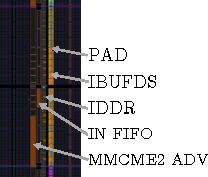
\includegraphics[width=0.4\textwidth]{figures/adc_input_bank}
  \caption{View of the Physical Location of the Primitives forming the
    \gls{ADC} Interface on the \gls{FPGA}}
  \label{fig:adc_input_bank}
\end{figure}

\subsection{Stage 3: Centralization and Reordering}
\label{sec:fpga_adc_s3}
All previous stages kept the four input streams separated
and were placed close to four input banks spread across the whole die.
Hence the data has to be routed to one place first.
This is done by allocating three \gls{req}/\gls{ack}-breakers
in series for each of the four channels.
This induces a high flexibility to the tools in allocating routing
resources and putting registers in between. \\

The four last \gls{req}/\gls{ack}-breakers of the four channels are then connected
to one single \gls{req}/\gls{ack}-breaker which forms the final output of the
\gls{ADC} module. The data is ordered in such a way, that the final 192 bit
wide output vector is formatted as follows:
\[Q_7\;I_7\;Q_6\;I_6\;Q_5\;I_5\;Q_4\;I_4\;Q_3\;I_3\;Q_2\;I_2\;Q_1\;I_1\;Q_0\;I_0\]
Where $Q_t$ and $I_t$ are the quadrature channel respectively in-phase channel
12 bit words at time $t$.
The index $t$ is the time step. A higher number means later in time.
All words are formatted with \gls{MSB} first. \\

This results in a $1 \times 192$ bits, single ended, single data rate signal. \\

\subsection{Test Pattern Generator}
For debugging purposes, the \gls{ADC} interface has a built in test pattern
generator which outputs 16 words of 12 bit numbers in parallel, such that
when lining them up to 192 bit vectors this results in a continuous count.

\section{High Speed Data Storage}
\label{sec:fpga_storage}

Whenever a positive edge is detected on the trigger input or the trigger
button is pressed, the \gls{RAM} is completely overwritten with a new run of
\gls{ADC} samples. \\

The arm signal (see \figref{fig:fpga_architecture_overview}) is deasserted
by the \gls{MB} processor while a download operation is in process
(see \secref{sec:fpga_download}) to avoid mixing up multiple runs. \\

The used \gls{RAM} module MT8JTF1286Hz is a standard \acrshort{DDR}3 \gls{RAM}
and offers a total of 1 GiB of space spread across 8 banks of 128 MiB each.
This allows for parallel data transfers of 64 bits at speed of up to 800 MHz
resulting in a maximal bandwidth of $12.8 \text{GB}/\text{s}$. \\

Very similar to the \gls{ADC} data acquisition module (\secref{sec:fpga_adc})
this high clock rates can only be used very close to the \gls{IO} banks
and not for further routing and processing in the \gls{FPGA}.
For that purpose Xilinx provides a \gls{IP} core that on one end is connected
to the pads of the \gls{RAM} module and on the other side offers a user
friendly \gls{UI} on a slower clock frequency.
It does so by taking care of address generation, refreshing the volatile
memory and scheduling read and write options. \\

Because place \& route turned out to be difficult at the maximal speed
of 800 MHz, 500 MHz is used as \gls{RAM} clock rate.
When configuring the core to use a 1:4 multiplexing, the \gls{UI} runs
at 125 MHz, has a $4 \cdot 2 \cdot 64 = 512$ bits wide data bus
and a maximal bandwidth of $8 \text{GB}/\text{s}$. This is still slightly
higher than bandwidth of the \gls{ADC} and therefore allows real-time
storage of all data. Since there is 1 GiB \gls{RAM}
a total of $\approx 3.6 \cdot 10^8$ complex samples can be saved. This
takes $\approx 190 \text{ms}$ at full \gls{ADC} speed. \\

Experiments showed that it is possible to consecutively writing to all
addresses without the \gls{MIG} core stalling for refresh operations.
Whenever, during a write request, one sole read request
is performed, the \gls{UI} of the \gls{MIG} core stalls for about 11
cycles. This is not an issue as in our case we first write
to all addresses, then stop writing and read out a part of the memory
at much lower speeds (see \secref{sec:fpga_download}). \\

Since the \gls{ADC} module outputs the data at 250 MHz in a 192 bit
wide vector and the \gls{RAM} module can write 512 bit wide vectors
at only 125 MHz, a bus converter is used which concatenates 192 bits
words until at least 512 bits are available. Behind this converter
a \gls{FIFO} memory is added to cross the clock boundary and to be able
to hold some samples when the \gls{MIG} user interface stalls. \\

During implementation, care has to be taken to the mask bits,
which are designed to prevent parts of the 64 bits written in parallel to be
overwritten and therefor allow for partial writes without first performing
a read operation. Accidentally having these pins stuck at 1 due to
not connecting them prevents initialization and further reads from
working. \\

\section{Download}
\label{sec:fpga_download}
For further analysis and processing of the data captured by the \gls{ADC},
it is sent to a personal computer.
Different options for downloading the 1 GiB of data from the \gls{FPGA}
to a computer were considered: \\

The simplest implementation would be to use the CP2103GM
\acrshort{USB}-to-\acrshort{UART} bridge \gls{IC} soldered on the VC707.
Since it's baud rate is limited to $1 \text{Mbit}/\text{s}$
a complete download of 1 GiB would take about 18 minutes which was
considered to be too slow. \\

Next the Tri-Speed Ethernet \gls{PHY} device was considered.
The high data rates of up to $1 \text{Gbit}/\text{s}$ and the versatility
of being able to connect it to existing network infrastructure made
it look perfect for the job. The lack of a good reference design and
availability of open cores to connect to the \gls{PHY} via
\gls{SGMII} as well as the effort needed to implement
the network and transport (\gls{INetP}/\gls{UDP}) layer
led to the third solution. \\

The VC707 also includes a USB3320 USB 2.0 ULPI device and Xilinx provides
a \gls{IP} core to connect to it. The theoretical maximal
raw bandwidth of $60 \text{MB}/\text{s}$ would allow for a relatively fast
download. Also \gls{USB} is very common way to connect to modern laboratory
equipment.

\subsection{Microblaze Soft-core processor}
Since the initialization, control logic and packet formatting
used to implement the \gls{USB} slave device can much easier be implemented
in software than using look-up tables and \glspl{FSM} a
\gls{MB} soft-core processor was configured into the \gls{FPGA}. \\

The \gls{MB} processor uses a \gls{AXI} bus to communicate with the following
peripherals:
\begin{itemize}
\item RS232 \gls{UART} for status and debug outputs
\item 4 Bit output to control debug \glspl{LED}
\item USB 2 controller
\item An interrupt controller
\item The custom receiver peripheral
\end{itemize}

Since the \gls{RAM} module had to be optimized for best write performance
as described in \secref{sec:fpga_storage} not the standard Xilinx \gls{IP}
core to interface the \gls{MIG} core to the \gls{AXI} bus was used.
Instead a custom \gls{AXI} peripheral was implemented which allows to
control and monitor the data acquisition and a second peripheral allows
for memory mapped read access of the \gls{RAM} by the \gls{MB}. \\

For simplicity the \gls{DMA} unit of the \gls{USB} peripheral was not used.
Instead the data was first read from the custom peripheral
by the \gls{MB} processor and then written to \gls{USB} peripheral.
This allows for data transfer rates of about $16 \;\text{MB} / \text{s}$
which is already fast enough. \\

\subsection{Communication Protocol}
To manage the communication between the host computer and the \gls{USB} device
implemented by the \gls{MB} processor a simple protocol was defined.
It involves 5 endpoints as defined by the \gls{USB}2 standard.
Only the Hi-Speed mode of \gls{USB}2 is supported. The slower Full Speed mode
is not supported. \\

Endpoint 0 is a standardized control endpoint. It's purpose is to
enumerate the bus\footnote{give the slave a unique address} and to provide the
host computer with information about basic parameters and the other endpoints.
It's exact behaviour is defined by the
``Chapter 9 USB Device Framework'' of the \gls{USB}2 standard \todo{add reference}. \\

Endpoint 1 is used to transfer binary raw data from the computer to the \gls{FPGA}
while endpoint 2 does the same into the other direction. They both use the maximal
possible packet size of 512 byte in bulk transfer mode. \\

Endpoint 3 is used in bulk mode to transfer short binary requests used to
initiate data transfers by allowing to set a write address pointer,
to set a read address pointer and to request a number of blocks to receive. \\

Finally endpoint 4 is used in bulk mode to respond to the requests sent
to endpoint 3 with either a success or an error code and to receive information
about the current read / write pointers and the amount of available memory. \\

\subsection{Computer Software}
In order to download the samples from the \gls{FPGA} in Matlab, a small
middleware (about 400 lines of C code) was written.
It depends on libusb \todo{add reference} and sends the necessary commands
to download all or part of the memory content.
The data consisting of 12 bit words is then zero-padded to 16 bit words
and written to a binary file which can be read very fast in Matlab. \\

\begin{figure}[ht]
  \centering
  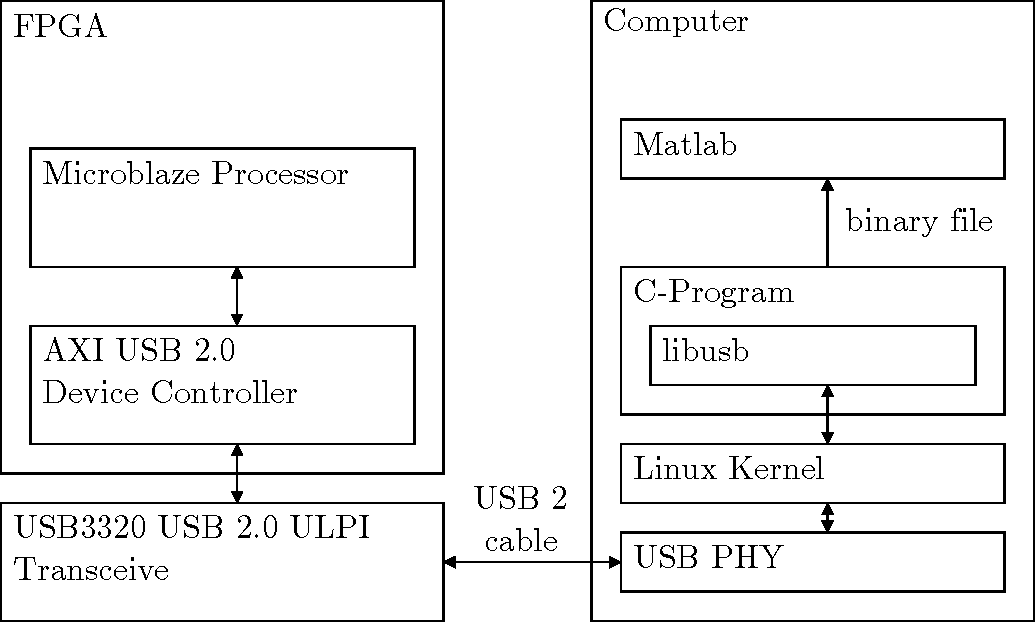
\includegraphics[width=0.6\textwidth]{figures/fpga_download}
  \caption{Overview of Download Process}
  \label{fig:fpga_download}
\end{figure}

\section{Clock Domains}
\label{sec:fpga_clocks}

As a result of the different clocking constraints of the externals interfaces,
a relatively complex clocking scheme had to be applied as drawn in
\figref{fig:fpga_clock_domains}. Except for parts of the \gls{IO} interfaces,
synchronous positive edge triggered registers were used. For the synchronization
of the data paths crossing clock boundaries the numerous FIFO36E1 primitives
were used. Those configure the block \gls{RAM} cells to act as a \gls{FIFO}
memory. A wrapper is used to connect multiple of those primitives 
in parallel to allow for the wide vectors of up to 540 bits.
An exception are the \gls{ADC} and \gls{RAM} blocks which use
specialized \gls{INFIFO} and OUT\_FIFO, which can do a 1:2 de-/multiplexing
using two independent input and output clocks. \\

\figref{fig:fpga_clock_generation} shows all the \glspl{PLL} used to derive the
different clocks. Because the \gls{MIG} core designed by Xilinx includes
it's own \gls{PLL} which optimally is directly connected to an external
clock source, the \gls{LVDS} signal of the SiT9102 200 MHz Fixed Frequency
Oscillator is directly connected to the \gls{PLL} inside the \gls{MIG} core.
The derived 125 MHz \gls{RAM} \gls{UI} clock is than used by the main
\gls{PLL} to derive all needed clocks for the peripheral. \\

In the following sections the clocking constraints of the different modules
are described. The closely related reset implementation is described
in \secref{sec:fpga_reset}. \\

\subsection{\gls{ADC}}
The \gls{ADC} provides a clock parallel to each of the four data streams.
The four clocks I0 Clk, I1 Clk, Q0 Clk and Q1 Clk are shown on
\figref{fig:fpga_architecture_overview} and are referred to as \gls{ADC} clocks.
They can be up to 450 MHz (1.8 $\text{GS}/\text{s}$ \gls{DDR})
and also significantly slower for slow (e.g. 800 $\text{MS}/\text{s}$)
sampling rates. \\

Each differential \gls{ADC} clock is first converted to a single ended
clock and than fed into a \gls{PLL} located next to the corresponding input
bank. This \gls{PLL} outputs a new clock in a local clock region
with the same frequency but an arbitrary phase shift
to clock the \gls{IDDR} and \gls{INFIFO} as described in \secref{sec:fpga_adc}.
Since the edges of the \gls{ADC} clocks and the corresponding data lines
are aligned, a phase shift of $90^\circ$ was found to work well and captures
the data during the stable period. \\

After parallelisation, a new clock domain, the \gls{ADC} \gls{UI} clock
is used to do the centralization and reordering,
to do the bus conversion and finally to put the data into a \gls{FIFO}
traversing to the clock region of the \gls{RAM} \gls{UI} described
in \secref{sec:fpga_storage}. This clock has to be strictly greater than
$\frac{900\;\text{MHz}}{4} = 225\;\text{MHz}$ to avoid the
\gls{INFIFO} from filling up. Also there needs to be a minimal
distance between an edge of the \gls{ADC} \gls{UI} and the
\gls{RAM} \gls{UI} clock in order for the FIFO36E1 to work correctly.
Hence a clock rate of 250 MHz was chosen. \\

\subsection{\gls{RAM}}
\label{sec:fpga_clock_ram}
The used \gls{DDR} \gls{RAM} module can be clocked up to 800 MHz which would
allow for a data rate of
$2 \cdot 64\;\text{bit} \cdot 800\;\text{MHz} = 12.8 \text{GB} / \text{s}$.
As described in \secref{sec:fpga_storage}, a lower frequency of 500 MHz
was chosen. To allow interfacing the \gls{MB} at a as low as possible speed,
the \gls{MIG} core was configured to use an internal 1:4 multiplexing. This results
in \gls{RAM} \gls{UI} clock of 125 MHz.

\subsection{\acrfull{MB}}
Finally, the \gls{MB} processor described in \secref{sec:fpga_download} has
it's own clock running at 100 MHz. \\

Later test runs showed, that the warning of the Platform studio saying that the
\gls{MB} runs only up to 100 MHz could be ignored and the \gls{MB} including
the \gls{USB} interface can run at 125 MHz as well. This removes one clock boundary
and slightly increases the download speed by faster copying data from the
\gls{RAM} to the \gls{USB} buffer. \\

\begin{figure}
  \centering
  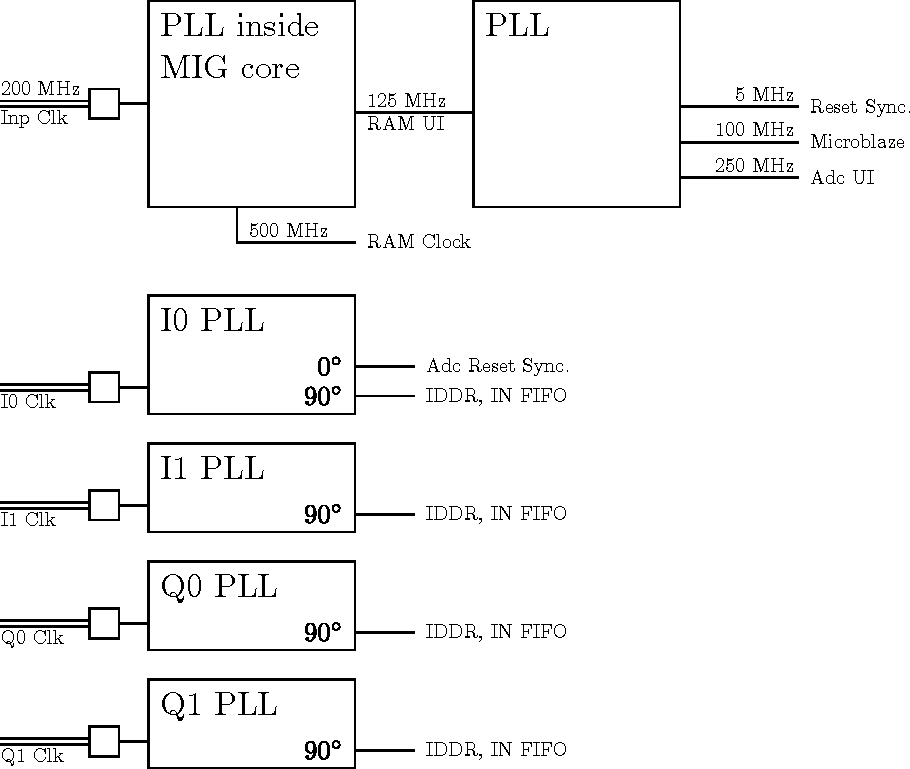
\includegraphics[width=0.7\textwidth]{figures/clock_generation}
  \caption{Block Diagram of Clock Generation}
  \label{fig:fpga_clock_generation}
\end{figure}

\begin{figure}
  \centering
  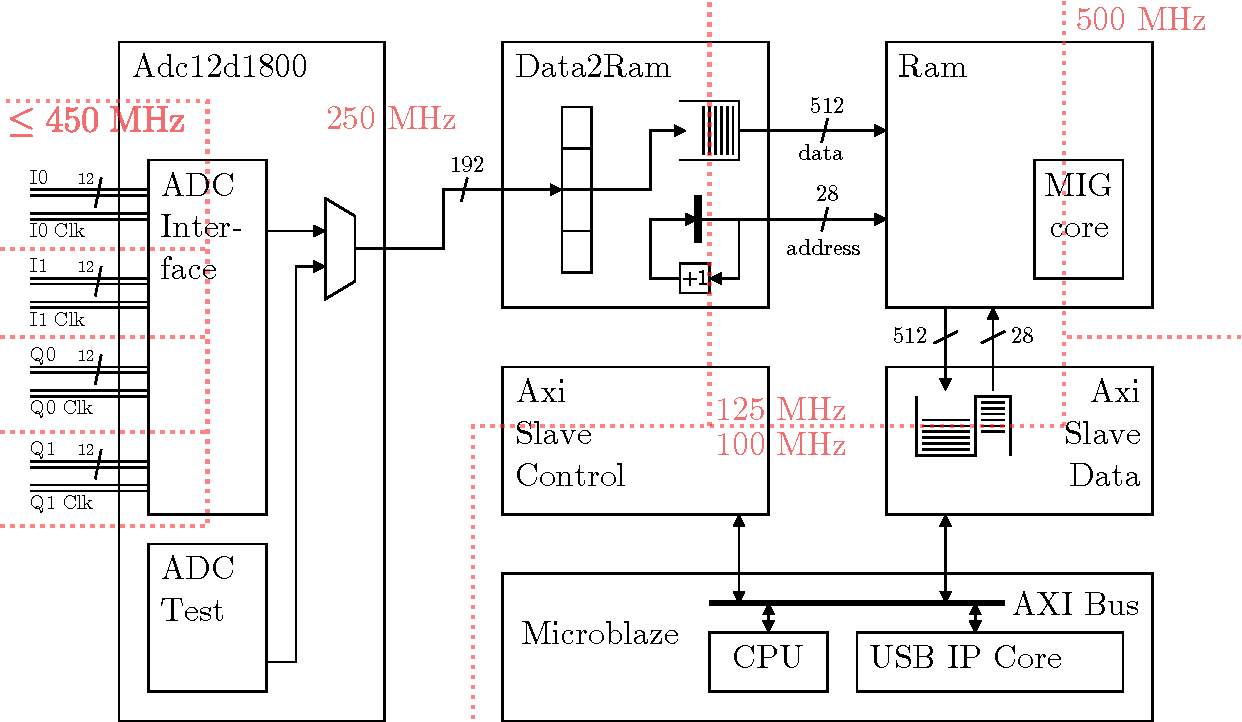
\includegraphics[width=\textwidth]{figures/fpga_clock_domains_overview}
  \caption{Overview of Clock Domains}
  \label{fig:fpga_clock_domains}
\end{figure}

\section{Reset Distribution}
\label{sec:fpga_reset}

In consequence of all those clocking regions, implementing a correct
reset scheme turned out to be trickier than one might think. \\

In general, high active, asynchronous resets were implemented for all
registers. Whenever a clock boundary had to be crossed, a reset synchronizer
as shown in \figref{fig:fpga_rst_sync} was used. The first register
makes sure the reset is release synchronous to the positive clock edge
of the target clock, in order to have a full clock period to distribute
the reset signal to all target registers. The second register is
to make sure the possible meta stability problems of the first registers would
no propagate. Clock and reset distribution networks both need to
distribute a signal with a limited amount of jitter and skew to a possibly
high fan-out. Therefor the same routing resources and buffers can be used.  \\

An overview of the reset distribution is given in
\figref{fig:fpga_rst_generation}. The reset can be triggered
by an external button or by the general reset of the \gls{FPGA}
used while downloading the bit file. Because the main system clock is
not available during reset, the reset button input is debounced using a
156 MHz clock generated by a second oscillator on the VC707 board.
When the reset is released, first the \gls{MIG} core starts
it's \gls{PLL}, needs some time to initialize the \gls{RAM} and than
outputs a initialization complete signal which is used to derive the main reset
for the rest of the logic including the \gls{MB} and \gls{ADC} modules.
This main reset signal is than first synchronized to 5 MHz which is a
integer divider of all clocks and therefore is only released synchronous
to all clocks. \\

The very long setup time of the synchronous reset input of the FIFO36E1
can only be met at 240 MHz if there is a reset synchronization register
close to the FIFO primitive.
Therefor two global, 5 MHz synchronous reset networks are globally distributed.
The normal master reset used for all logic except
for the FIFO36E1 primitives and a second, two clock cycles earlier, reset signal.
An additional reset synchronizer, connected to the earlier reset,
prevented from being trimmed away by logic optimization and without 
output buffer is placed next to each FIFO36E1 primitive. \\

Another challenge was to correctly reset the \gls{INFIFO} used in the
\gls{ADC} module as described in \secref{sec:fpga_adc}. These \glspl{FIFO}
cross the boundary between the clock regions provided by the \gls{ADC} and
the internal 250 MHz clock. The 4 clocks of the 4 channels might
have a slightly different phase, are derived from the same clock, the
\gls{ADC} sampling clock, though. It is crucial to release the reset
of all \gls{INFIFO} during the same \gls{ADC} sampling clock period to avoid
misalignment of the data. For that purpose, the global 5 MHz
reset is first synchronized to a $90^\circ$ phase shifted version of I0's clock
and than synchronized to the four \gls{ADC} clocks. \\

\begin{figure}
  \centering
  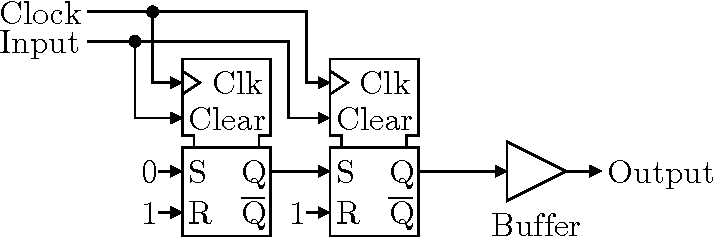
\includegraphics{figures/RstSync}
  \caption{Reset Synchronizer used to cross clock domains}
  \label{fig:fpga_rst_sync}
\end{figure}

\begin{figure}
  \centering
  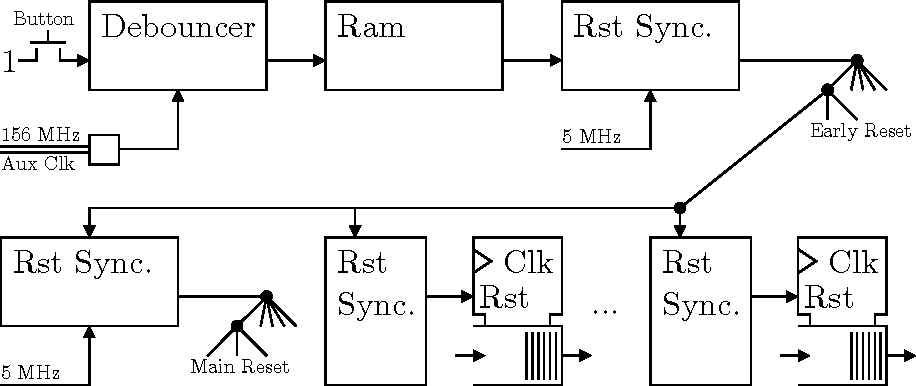
\includegraphics[width=0.7\textwidth]{figures/rst_generation}
  \caption{Overview of the Reset Distribution}
  \label{fig:fpga_rst_generation}
\end{figure}

\section{Tools \& Development flow}
\label{sec:fpga_tools}

The \gls{FPGA} design and it's software consists of three different
main parts: \\

First the \gls{ADC} interface, the \gls{RAM} and the connecting
glue logic were implemented.
This part was fully developed using the Xilinx ISE 14.4
design suite. For testing an debugging manually inserted ChipScope
instruments were used, which form a logic analyzer running on the \gls{FPGA}
alongside the other modules. Since these instruments shares the same logic,
memory and routing resources, they heavily influence the mapping and routing
of the logic and therefor the timing of the circuit, which can make debugging
timing problems cumbersome. \\
This project than interfaces directly to many externals pins and implements
the \gls{AXI} bus interface, which was tied to dummy inputs for synthesis in
ISE. \\

In a second step, Xilinx Platform Studio, which is part of the Xilinx
\gls{EDK} 14.4, was used to create a project build around the \acrfull{MB}
soft-core processor. The ISE project consisting of the \gls{ADC} and \gls{RAM}
interface forms a peripheral. \\

In a third step, the software running on the \gls{MB} processor had to be
developed. This was done using Emacs and the Xilinx \gls{EDK} tools
consisting mainly of an Eclipse plugin. \\

The development process, of course, was not linear. These three steps were
iterated over multiple times. A complete run of synthesis, map,
place \& route, timing analysis and bit file generation
took between 20 minutes and 2 hours depending on how tight the timing was
and on how big the memory of the ChipScope instruments were chosen.
Since especially the debugging of the \gls{RAM} module and the implementation of
a correct reset behaviour (see \secref{sec:fpga_reset}) included a lot of
trial \& error, dozens of \gls{CPU} and man hours were spent on the
compiling the design.

%%  LocalWords:  FPGA Virtex VC Matlab DDR fpga Adc Microblaze AXI rf
%%  LocalWords:  AxiSlave Req Ack stallable req ack LUT virtex FMC ns
%%  LocalWords:  adc ASIC CMOS LVDS parallelised parallelise IBUFDS
%%  LocalWords:  parallelisation IDDR Xilinx MMCME MSB deasserted JTF
%%  LocalWords:  GiB MiB IP UI CP UART IC Mbit Tri PHY Gbit SGMII UDP
%%  LocalWords:  INetP ULPI FSM DMA middleware libusb de PLL SiT Clk
%%  LocalWords:  synchronizer rst jitter debounced synchronizers ISE
%%  LocalWords:  ChipScope EDK INFIFO
